\documentclass[12pt]{article}
\usepackage[utf8]{inputenc, }
\usepackage{graphicx}
\usepackage{hyperref}
\usepackage[margin=1in]{geometry}
\usepackage{setspace}
\usepackage{color}
\usepackage{pdfpages}
\usepackage{amsmath}
\usepackage{amsfonts}
\usepackage{float}
\usepackage{tikz}
\usepackage{pgfplots}
\usepackage{enumitem}
\usepackage{xpatch}
\usepackage{svg}
\usepackage{mathrsfs}
\usepackage{steinmetz}
% \usepackage[nocheck]{fancyhdr}

\sloppy
\definecolor{lightgray}{gray}{0.5}
\setlength{\parindent}{0pt}

\hypersetup{
    colorlinks,
    citecolor=black,
    filecolor=black,
    linkcolor=black,
    urlcolor=black
    pdftitle={EE300 İsmail Enes Bülbül}
}
\onehalfspacing

% \raggedright

\title{EE301 Homework-3}
\author{İsmail Enes Bülbül, Eren Meydanlı, Ahmet Caner Akar}
%\date{October 2022}
\renewcommand*\contentsname{Table of Contents}
\renewcommand*{\refname}{}
% \fancyhf{} % sets both header and footer to nothing
% \renewcommand{\headrulewidth}{0pt}
\begin{document}

\maketitle
% \tableofcontents
% \newpage

    \section*{Question 1}
    \subsection*{a)}
    The magnitude and phase responses of \(H(j\omega)\) can be seen below:
\begin{center}
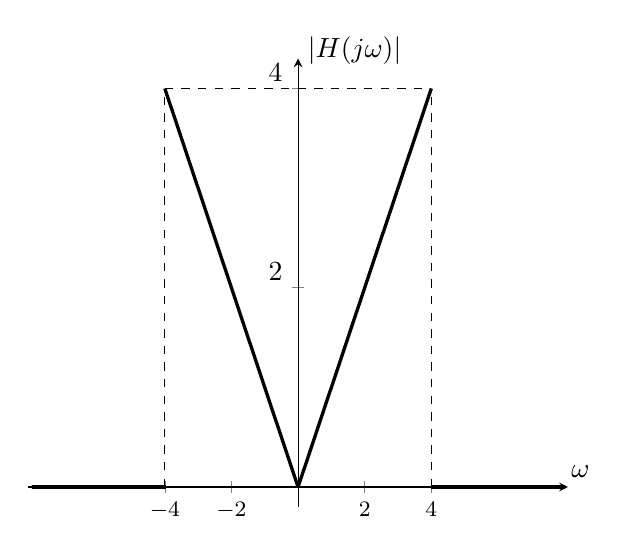
\begin{tikzpicture}
\begin{axis}[
    axis lines = middle,
    ymin = -0.2,
    ymax = 4.3,
    xmax = 8.1,
    xmin = -8.1,
    xlabel = \(\omega\),
    xlabel style={xshift=0.4cm},
    ylabel style={yshift=0.4cm},
    ylabel = {\(|H(j\omega)|\)},
    xtick={-4, -2, 0, 2, 4},
    xticklabel style={font=\footnotesize,fill=white},
    yticklabel style={yshift=0.2cm},
    ytick={0,2,4},
    samples=500,
    ]
        \addplot [domain=-4:0,style=very thick,black] {-x};
        \addplot [domain=0:4,style=very thick,black] {x};
        \addplot [domain=-8:-4,style=very thick,black] {0};
        \addplot [domain=4:8,style=very thick,black] {0};
        \draw[dashed] (axis cs: -4,0)--(axis cs: -4,4);
        \draw[dashed] (axis cs: 4,0)--(axis cs:  4,4);
        \draw[dashed] (axis cs: -4,4)--(axis cs:  4,4);
\end{axis} 
\end{tikzpicture}
\end{center}
\begin{center}
\begin{tikzpicture}
 \begin{axis}[
    axis lines = middle,
    xmax = 4,
    xmin = -4,
    xlabel = \(\omega\),
    xlabel style={xshift=0.4cm},
    ylabel style={yshift=0.4cm},
    ylabel = {\(\phase{H(j\omega)}\)},
    xtick={-4, -2, 0, 2, 4},
    xticklabel style={font=\footnotesize,fill=white},
    yticklabel style={font=\footnotesize,fill=white,yshift=0.2cm},
    ytick={-90,-45,0,45,90},
    yticklabels={$-90^{\circ}$,$-45^{\circ}$,,$45^{\circ}$,$90^{\circ}$},
    samples=500,
    enlargelimits=true,
    ]
        \addplot [domain=-4:0,style=very thick,black] {-90};
        \addplot [domain=0:4,style=very thick,black] {90};
        \draw[dashed] (axis cs: -4,0)--(axis cs: -4,-90);
        \draw[dashed] (axis cs: 4,0)--(axis cs:  4,90);
\end{axis} 
\end{tikzpicture}
\end{center}
    \subsection*{b)}
    \section*{Question 2}
    \subsection*{a)}
    We know that \(X(j\omega) = \int_{\infty}^{-\infty} x(t)e^{-j\omega t} \,dt \). Then\\
    \begin{math}
      \frac{d}{d\omega} X(j\omega) = \frac{d}{d\omega} \int_{\infty}^{-\infty} x(t)e^{-j\omega t} \,dt
      =\int_{\infty}^{-\infty} \frac{d}{d\omega}(x(t)e^{-j\omega t}) \,dt = \int_{\infty}^{-\infty} x(t)(-jt)e^{-j\omega t} \,dt
      =\mathscr{F}\{x(t)(-jt)\}
    \end{math}\\
    Therefore, \(\mathscr{F}^{-1}\{\frac{d}{d\omega} X(j\omega)\}=x(t)(-jt)\)
    \subsection*{b)}
    Let \(g_1(t) = \frac{sin(\pi t)}{\pi t}\). Then we know that \(\mathscr{F}\{g_1(t)\} = \begin{cases}
    1,& |\omega| < \pi\\
    0,& else\\
    \end{cases}\)\\
    Since \(g(t) = g_1(t)g_1(t)\), by multiplication property, we know that \(G(j\omega) = \frac{1}{2\pi}G_1(j\omega)*G_1(j\omega)\)\\
    \begin{math}
      G(j\omega) = \frac{1}{2\pi}\int_{-\infty}^{\infty} G(j\theta)G(j(\omega-\theta)) \,d\theta
      = \frac{1}{2\pi}\int_{-\pi}^{\pi} G(j(\omega-\theta)) \,d\theta 
    \end{math}\\
    Let \(\theta' = \omega - \theta\). Then \(d\theta' = -d\theta\) and\\
    \begin{math}
      G(j\omega) = \frac{1}{2\pi}\int_{\omega+\pi}^{\omega-\pi} G_1(j\theta') \,d(-\theta')
      = \frac{1}{2\pi}\int_{\omega-\pi}^{\omega+\pi} G_1(j\theta') \,d\theta'
    \end{math}\\
    For \(\omega < -2\pi\) or \(\omega > 2\pi\), \(G(j\omega) = 0\).
    For \(\omega < 0\)\\
    \begin{math}
      G(j\omega) = \frac{1}{2\pi}\int_{-\pi}^{\omega+\pi}  \,d\theta' = \frac{\omega+\pi}{2\pi}
    \end{math}\\
    For \(\omega > 0\)\\
    \begin{math}
      G(j\omega) = \frac{1}{2\pi}\int_{\omega-\pi}^{\pi}  \,d\theta' = \frac{2\pi-\omega}{2\pi}
    \end{math}\\
    Therefore, \(G(j\omega) =\begin{cases}
      \frac{\omega+\pi}{2\pi},& -2\pi < \omega < 0\\
      \frac{2\pi-\omega}{2\pi},& 0 < \omega < 2\pi\\
      0,& else\\
      \end{cases}\), and \(G(j\omega)\) is plotted below\\
    \begin{center}
      \begin{tikzpicture}
        \begin{axis}[
            axis lines = middle,
            ymin = 0,
            ymax = 1/pi,
            xmax = 7,
            xmin = -7,
            xlabel = \(\omega\),
            xlabel style={xshift=0.4cm},
            ylabel style={yshift=0.4cm},
            ylabel = {\(G(j\omega)\)},
            xtick={-2*pi,0,2*pi},
            xticklabels={$-2\pi$,$2\pi$},
            xticklabel style={font=\footnotesize,fill=white},
            yticklabel style={yshift=0.2cm},
            ytick={0,1/(2*pi)},
            yticklabels={$1\(2pi)$},
            samples=500,
            ]
                \addplot [domain=-2*pi:0,style=very thick,black] {(x+2*pi)/(2*pi)};
                \addplot [domain=0:2*pi,style=very thick,black] {(2*pi-x)/(2*pi)};
                \addplot [domain=-7:-2*pi,style=very thick,black] {0};
                \addplot [domain=2*pi:7,style=very thick,black] {0};
                % \draw[dashed] (axis cs: -4,0)--(axis cs: -4,4);
                % \draw[dashed] (axis cs: 4,0)--(axis cs:  4,4);
                % \draw[dashed] (axis cs: -4,4)--(axis cs:  4,4);
        \end{axis} 
        \end{tikzpicture}
    \end{center}
    \subsection*{c)}
    \subsubsection*{i)}
    \begin{math}
      H(j\omega) = \int_{-\infty}^{\infty} f^*(-t)e^{-j\omega t} \,dt 
      = \int_{-\infty}^{\infty} (f(-t)e^{j\omega t})^* \,dt 
    \end{math}\\
    Let \(t' = -t\). Then \(dt'=-dt\) and \\
    \begin{math}
      H(j\omega) = \int_{\infty}^{-\infty} (f(t')e^{-j\omega t'})^* \,d(-t')
      = \int_{-\infty}^{\infty} (f(t')e^{-j\omega t'})^* \,d(t')
      = (\int_{-\infty}^{\infty} f(t')e^{-j\omega t'} \,d(t'))^*
      = F^*(j\omega) 
    \end{math}
    \subsubsection*{ii)}
    Let \(\mathscr{F}\{y(t)\} = Y(j\omega)\). Then \(Y(j\omega) = F^*(j\omega)F(j\omega) = |F(j\omega)|^2\)\\
    \begin{math}
      y(t) = \frac{1}{2\pi} \int_{-\infty}^{\infty} Y(j\omega)e^{j\omega t} \,d\omega
      =
    \end{math}
    \section*{Question 3}
    \subsection*{a)}
    \subsubsection*{i)}
    \begin{math}
    x(t) = \frac{sin(4\pi t)}{\pi t} cos(2\pi t) = \frac{4sin(4\pi t)}{4\pi t} cos(2\pi t) = x_1(t)x_2(t) \left(\textrm{ where }x_1(t) = \frac{4sin(4\pi t)}{4\pi t} \textrm{, } x_2(t) = cos(2\pi t)\right)\\ \\ 
    \textrm{Recall that: } \mathscr{F}\{rect(\theta)\} = \frac{sin(\omega/2)}{\omega/2} \\
    \textrm{By duality property of CTFT: }\frac{sin(t/2)}{t/2} \longleftrightarrow 2\pi rect(-\omega) = 2\pi rect(\omega) \\
    \textrm{By scaling property of CTFT: }\frac{sin(4\pi t)}{4\pi t} \longleftrightarrow \frac{rect(\frac{\omega}{8\pi})}{4} \\
    \textrm{By linearity: } \frac{4sin(4\pi t)}{4\pi t} \longleftrightarrow rect(\frac{\omega}{8\pi}) = X_1(j\omega) \\ \\
    x_2(t) = cos(2\pi t) = \frac{1}{2} e^{j2\pi t} + \frac{1}{2} e^{-j2\pi t} \\
    \mathscr{F}\{\frac{1}{2} e^{j2\pi t} + \frac{1}{2} e^{-j2\pi t}\} \longleftrightarrow \pi [\delta(\omega+2\pi) + \delta(\omega-2\pi)] = X_2(j\omega) \\ \\
    \textrm{By modulation property of CTFT: } \\
    x(t) = x_1(t) x_2(t) \longleftrightarrow X(j\omega) = \frac{1}{2\pi} X_1(j\omega)*X_2(j\omega) \\
    X(j\omega) = \frac{1}{2\pi} rect(\frac{\omega}{8\pi})*\pi [\delta(\omega+2\pi) + \delta(\omega-2\pi)] = \frac{1}{2} [rect(\frac{\omega}{8\pi})*\delta(\omega+2\pi) + rect(\frac{\omega}{8\pi})*\delta(\omega-2\pi)] \\
    X(j\omega) = \frac{1}{2} rect(\frac{\omega+2\pi}{8\pi}) + \frac{1}{2} rect(\frac{\omega-2\pi}{8\pi}) 
    \end{math} \\
    \begin{center}
  \begin{tikzpicture}
\begin{axis}[
    axis lines = middle,
    ymin = -0.2,
    ymax = 1.1,
    xlabel = \(\omega\),
    xlabel style={xshift=0.4cm},
    ylabel style={yshift=0.4cm},
    ylabel = {\(X(j\omega)\)},
    xtick={-6*pi, -4*pi, -2*pi, 0, 2*pi, 4*pi, 6*pi},
    xticklabel style={font=\footnotesize,fill=white},
    yticklabel style={yshift=0.2cm},
    xticklabels={$-6\pi$,$-4\pi$,$-2\pi$,,$2\pi$,$4\pi$,$6\pi$},
    ytick={0,0.5,1},
    samples=500,
    enlargelimits=true,
    ]
        \addplot [domain=-6*pi:-2*pi,style=very thick,black] {0.5};
        \addplot [domain=-2*pi:2*pi,style=very thick,black] {1};
        \addplot [domain=2*pi:6*pi,style=very thick,black] {0.5};
        \draw[dashed] (axis cs: 2*pi,0)--(axis cs: 2*pi,1);
        \draw[dashed] (axis cs: -2*pi,0)--(axis cs: -2*pi,1);
        \draw[dashed] (axis cs: 6*pi,0)--(axis cs: 6*pi,0.5);
        \draw[dashed] (axis cs: -6*pi,0)--(axis cs: -6*pi,0.5);
        \draw[dashed] (axis cs: -2*pi,0.5)--(axis cs: 2*pi,0.5);
\end{axis}
\end{tikzpicture}
\end{center}
    \subsubsection*{ii)}
    \begin{math}
    y(t) = h(t)*x(t) \\
    \textrm{By convolution property of CTFT: } y(t) = h(t) * x(t) \longleftrightarrow Y(j\omega) = H(j\omega)X(j\omega)\\
    Y(j\omega) = \left(1-rect(\frac{\omega}{4\pi})\right)  \left(\frac{1}{2} rect(\frac{\omega-2\pi}{8\pi}) + \frac{1}{2} rect(\frac{\omega+2\pi}{8\pi})\right) \\
    Y(j\omega) = \frac{1}{2} rect(\frac{\omega-2\pi}{8\pi}) + \frac{1}{2} rect(\frac{\omega+2\pi}{8\pi}) - \frac{1}{2} \left(rect(\frac{\omega}{4\pi}) rect(\frac{\omega-2\pi}{8\pi})+ rect(\frac{\omega}{4\pi}) rect(\frac{\omega+2\pi}{8\pi})\right) \\
    Y(j\omega) = \frac{1}{2} \left(rect(\frac{\omega+4\pi}{4\pi}) + rect(\frac{\omega-4\pi}{4\pi})\right) \\
    \end{math}
    \begin{center}
  \begin{tikzpicture}
\begin{axis}[
    axis lines = middle,
    ymin = -0.2,
    ymax = 1.1,
    xlabel = \(\omega\),
    xlabel style={xshift=0.4cm},
    ylabel style={yshift=0.4cm},
    ylabel = {\(Y(j\omega)\)},
    xtick={-6*pi, -4*pi, -2*pi, 0, 2*pi, 4*pi, 6*pi},
    xticklabel style={font=\footnotesize,fill=white},
    yticklabel style={yshift=0.2cm},
    xticklabels={$-6\pi$,$-4\pi$,$-2\pi$,,$2\pi$,$4\pi$,$6\pi$},
    ytick={0,0.5,1},
    samples=500,
    enlargelimits=true,
    ]
        \addplot [domain=-6*pi:-2*pi,style=very thick,black] {0.5};
        \addplot [domain=-2*pi:2*pi,style=very thick,black] {0};
        \addplot [domain=2*pi:6*pi,style=very thick,black] {0.5};
        \draw[dashed] (axis cs: 2*pi,0)--(axis cs: 2*pi,0.5);
        \draw[dashed] (axis cs: -2*pi,0)--(axis cs: -2*pi,0.5);
        \draw[dashed] (axis cs: 6*pi,0)--(axis cs: 6*pi,0.5);
        \draw[dashed] (axis cs: -6*pi,0)--(axis cs: -6*pi,0.5);
        \draw[dashed] (axis cs: -2*pi,0.5)--(axis cs: 2*pi,0.5);
\end{axis}
\end{tikzpicture}
\end{center}
    \subsection*{b)}
    \subsubsection*{i)}
    By modulation property of CTFT: \\
    \begin{math}
    z(t) \longleftrightarrow Z(j\omega) = \frac{1}{2\pi} Y(j\omega) * \mathscr{F}\{\frac{sin(2\pi t)}{\pi t}\} =  \frac{1}{2\pi} Y(j\omega) * rect(\frac{\omega}{4\pi}) \\ 
    \Rightarrow Z(j\omega) = \frac{1}{2\pi} \left(rect(\frac{\omega+4\pi}{4\pi}) + rect(\frac{\omega-4\pi}{4\pi})\right) * rect(\frac{\omega}{4\pi}) \\
    \Rightarrow Z(j\omega) = \begin{cases}
        \frac{8\pi -\omega}{2\pi},& 4\pi< \omega < 8\pi \\
        \frac{\omega}{2\pi},&  0< \omega \leq 4\pi \\
        \frac{-\omega}{2\pi},&  -4\pi< \omega < 0 \\
       \frac{8\pi + \omega}{2\pi},&  -8\pi< \omega \leq -4\pi \\      
      \end{cases} 
    \end{math} 
    \begin{center}
  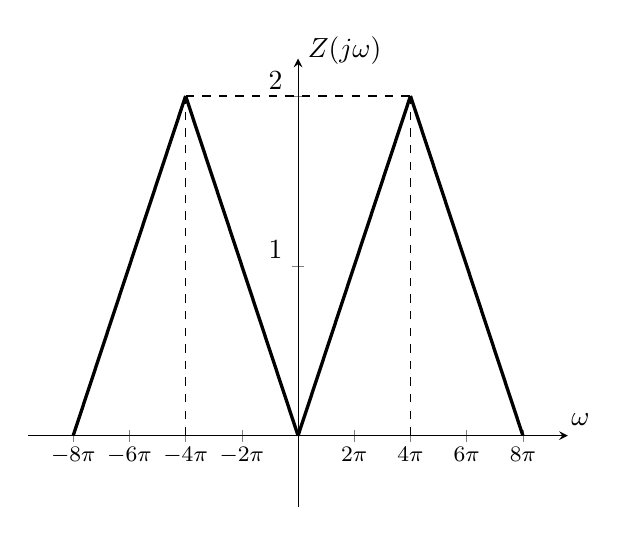
\begin{tikzpicture}
\begin{axis}[
    axis lines = middle,
    ymin = -0.2,
    ymax = 2,
    xlabel = \(\omega\),
    xlabel style={xshift=0.4cm},
    ylabel style={yshift=0.4cm},
    ylabel = {\(Z(j\omega)\)},
    xtick={-8*pi, -6*pi, -4*pi, -2*pi, 0, 2*pi, 4*pi, 6*pi, 8*pi},
    xticklabel style={font=\footnotesize,fill=white,inner sep=2pt},
    yticklabel style={yshift=0.2cm},
    xticklabels={$-8\pi$,$-6\pi$,$-4\pi$,$-2\pi$,,$2\pi$,$4\pi$,$6\pi$,$8\pi$},
    ytick={0,1,2},
    samples=500,
    enlargelimits=true,
    ]
        \addplot [domain=-8*pi:-4*pi,style=very thick,black] {(8*pi+x)/(2*pi)};
        \addplot [domain=-4*pi:0,style=very thick,black] {(-x)/(2*pi)};
        \addplot [domain=0:4*pi,style=very thick,black] {(x)/(2*pi)};
        \addplot [domain=4*pi:8*pi,style=very thick,black] {(8*pi-x)/(2*pi)};
        \draw[dashed] (axis cs: -4*pi,0)--(axis cs: -4*pi,2);
        \draw[dashed] (axis cs: 4*pi,0)--(axis cs: 4*pi,2);
        \draw[dashed] (axis cs: -4*pi,2)--(axis cs: 4*pi,2);
\end{axis}
\end{tikzpicture}
\end{center}
    \subsubsection*{ii)}
    \begin{math}
    y(t) \longleftrightarrow Y(j\omega) = rect(\frac{\omega+4\pi}{4\pi}) + rect(\frac{\omega-4\pi}{4\pi}) \\
    Y(j\omega) = \frac{1}{\pi} rect(\frac{\omega}{4\pi}) * \pi [\delta(\omega-4\pi) + \delta(\omega+4\pi)] \\
    \textrm{By modulation property of CTFT: } \\
    \mathscr{F}^{-1}\{Y(j\omega)\} = y(t) =  \frac{2sin(2\pi t)}{\pi t} cos(4\pi t) 
    \end{math} 
    \section*{Question 4}
    \subsection*{a)}
    \subsubsection*{i)}
    \begin{math} 
    X(e^{j\Omega}) = \displaystyle\sum_{n=-\infty}^{\infty} \underbrace{\delta[n] e^{-j\Omega n}}_{\delta[n] e^{-j\Omega 0}} = \displaystyle\sum_{n=-\infty}^{\infty} \delta[n] = 1 
    \end{math} 
     \subsubsection*{ii)}
    \begin{math} 
    X(e^{j\Omega}) = \displaystyle\sum_{n=-\infty}^{\infty} (2\delta[n-3] - \delta[n-10] ) e^{-j\Omega n} \stackrel{\text{(by linearity)}}{=} 2\displaystyle\sum_{n=-\infty}^{\infty} \delta[n-3] e^{-j\Omega n} - \displaystyle\sum_{n=-\infty}^{\infty} \delta[n-10] e^{-j\Omega n} \\ \\
    \textrm{By time-shift property of DTFT: } \\ 
    X(e^{j\Omega}) = 2e^{-j3\Omega} - e^{-j10\Omega} 
    \end{math} 
      \subsubsection*{iii)}
    \begin{math} 
    X(e^{j\Omega}) = \displaystyle\sum_{n=-\infty}^{\infty} x[n] e^{-j\Omega n} = \displaystyle\sum_{n=1}^{4} \frac{1}{n^{2}} e^{-j\Omega n} = e^{-j\Omega} + \frac{1}{4} e^{-j2\Omega} +\frac{1}{9} e^{-j3\Omega} + \frac{1}{16} e^{-j4\Omega}
    \end{math} 
     \subsubsection*{iv)}
    \begin{math}
    X(e^{j\Omega}) = \displaystyle\sum_{n=-\infty}^{\infty} \left(\left(\frac{1}{2}\right)^{n} u[n] - 3^{n} u[-n-1]\right)  e^{-j\Omega n} \\ 
    \stackrel{\text{(by linearity)}}{=}  \displaystyle\sum_{n=-\infty}^{\infty} \left(\frac{1}{2}\right)^{n} u[n] e^{-j\Omega n} - \displaystyle\sum_{n=-\infty}^{\infty} 3^{n} u[-n-1] e^{-j\Omega n} = \displaystyle\sum_{n=0}^{\infty} \left(\frac{1}{2} e^{-j\Omega}\right)^{n} - \displaystyle\sum_{n=-\infty}^{-1} 3^{n} e^{-j\Omega n} \\
    \displaystyle\sum_{n=0}^{\infty} \left(\frac{1}{2} e^{-j\Omega}\right)^{n} = \frac{1}{1- \frac{1}{2} e^{-j\Omega}} \quad \left(\textrm{since } \left\vert\frac{1}{2} e^{-j\Omega}\right\vert = \frac{1}{2} < 1, \textrm{so the expression is convergent}\right) \\ 
    \textrm{Let } m = -n: \displaystyle\sum_{n=-\infty}^{-1} 3^{n} e^{-j\Omega n} = \displaystyle\sum_{m=1}^{\infty} 3^{-m} e^{j\Omega m} = \displaystyle\sum_{m=1}^{\infty} \left(\frac{1}{3} e^{j\Omega}\right)^{m} = \underbrace{\left[\displaystyle\sum_{m=0}^{\infty} \left(\frac{1}{3} e^{j\Omega}\right)^{m}\right]}_{\frac{1}{1- \frac{1}{3} e^{j\Omega}}} -1 \\
    \Rightarrow X(e^{j\Omega}) = \frac{1}{1- \frac{1}{2} e^{-j\Omega}} - \left(\frac{1}{1- \frac{1}{3} e^{j\Omega}} -1\right)
    \end{math} 
    \subsubsection*{v)}
    Say that,  \begin{math} 
    \hat x[n] = \left(\frac{1}{2}\right)^{n} u[n] - 3^{n} u[-n-1]  \textrm{ and } \mathscr{F}\{\hat x[n]\}= \hat X(e^{j\Omega}) =  \frac{1}{1- \frac{1}{2} e^{-j\Omega}} - \left(\frac{1}{1- \frac{1}{3} e^{j\Omega}} -1\right)
    \end{math} \\ 
    By time-shift property of DTFT: \\ 
    \begin{math} 
    x[n] = \hat x[n-7] \longleftrightarrow X(e^{j\Omega}) = \hat X(e^{j\Omega}) e^{-j7\Omega}  \\ \\
    \Rightarrow X(e^{j\Omega}) = \frac{e^{-j7\Omega}}{1- \frac{1}{2} e^{-j\Omega}} - \left(\frac{e^{-j7\Omega}}{1- \frac{1}{3} e^{j\Omega}} -e^{-j7\Omega}\right)
    \end{math} 
    \subsubsection*{vi)}
    Let x[n] be a periodic signal with fundamental period N. Then, \\
    \begin{math}
    \mathscr{F}\{x[n]\} = X(e^{j\Omega}) = \displaystyle\sum_{m=-\infty}^{\infty} \displaystyle\sum_{k=k_0}^{k_0 + N-1} a_k 2 \pi \delta(\Omega -k \frac{2\pi}{N} - 2\pi m) \end{math} \\
    Note that for this signal if we consider the interval \(0 \leq \Omega < 2\pi \), DTFT of the signal will be written as: \\
    \begin{math}
    \mathscr{F}\{x[n]\} = X(e^{j\Omega}) = \displaystyle\sum_{k=0}^{2} a_k 2 \pi \delta(\Omega -k \frac{2\pi}{3}) \\
    \textrm{First, find the DTFS coefficients of x[n]: }  a_k = \frac{1}{3} \displaystyle\sum_{n=0}^{2} x[n] e^{-jk\frac{2\pi}{3}n}\\ 
    \Rightarrow a_0 = \frac{1}{3} \displaystyle\sum_{n=0}^{2} x[n] = \frac{1}{3} + \frac{1}{3} = \frac{2}{3} \\
    \Rightarrow a_1 = \frac{1}{3} \displaystyle\sum_{n=0}^{2} x[n] e^{-j\frac{2\pi}{3}n} = \frac{1}{3} e^{-j\frac{2\pi}{3}} + \frac{1}{3} e^{-j\frac{4\pi}{3}} =  \frac{-1}{3} \\ 
    \Rightarrow a_2 = \frac{1}{3} \displaystyle\sum_{n=0}^{2} x[n] e^{-j\frac{4\pi}{3}n} = \frac{1}{3} e^{-j\frac{4\pi}{3}} + \frac{1}{3} e^{-j\frac{8\pi}{3}} =  \frac{-1}{3} \\ \\   
    X(e^{j\Omega}) =  \displaystyle\sum_{k=0}^{2} a_k 2\pi \delta(\Omega -k \frac{2\pi}{3}) = a_0 2\pi \delta(\Omega) + a_1 2\pi \delta(\Omega - \frac{2\pi}{3}) + a_2 2\pi \delta(\Omega - \frac{4\pi}{3}) \\ 
     X(e^{j\Omega}) = \frac{2\pi}{3} \left(2 \delta(\Omega) - \delta(\Omega - \frac{2\pi}{3}) - \delta(\Omega - \frac{4\pi}{3})\right)
    \end{math} 
    
    \subsection*{b)}
    \subsubsection*{i)}
    \begin{math}
    x[n] = \frac{1}{2\pi} \displaystyle\int_{\Omega_0}^{\Omega_0 + 2\pi} \underbrace{X(e^{j\Omega})}_{=1} e^{j\Omega n} d\Omega = \frac{1}{2\pi} \displaystyle\int_{-\pi}^{\pi} e^{j\Omega n} d\Omega = \frac{1}{2\pi j n} \left(e^{j\pi n} - e^{-j\pi n}\right) \\
    x[n] = \frac{1}{\pi n} \frac{1}{2j} \left(e^{j\pi n} - e^{-j\pi n}\right) = \frac{sin(\pi n)}{\pi n} \qquad \boxed{\textrm{Recall that, } sinc(t) = \begin{cases}
        \frac{sin(\pi t)}{\pi t},& t \neq 0 \\
        1,& t=0\\
      \end{cases}}\\
      \textrm{Here, n is an integer. So, } \frac{sin(\pi n)}{\pi n} = \begin{cases}
        1,& n=0 \\
        0,& otherwise\\
      \end{cases} \Rightarrow x[n] = \delta[n] 
    \end{math}
    \subsubsection*{ii)}
    \begin{math}
    \textrm{We know that, } \mathscr{F}\{1\} =  2\pi \displaystyle\sum_{m=-\infty}^{\infty} \delta(\Omega - 2\pi m) \\
    \textrm{By frequency-shift property of DTFT: } \\
     \mathscr{F}\{e^{j\Omega_0 n}\} = 2\pi \displaystyle\sum_{m=-\infty}^{\infty} \delta(\Omega - \Omega_0 - 2\pi m) \\ 
    \Rightarrow \mathscr{F}\{e^{j\frac{\pi}{3}n}\} = 2\pi \displaystyle\sum_{m=-\infty}^{\infty} \delta(\Omega - \frac{\pi}{3} - 2\pi m) = 2\pi X(e^{j\Omega}) \\
    \Rightarrow \mathscr{F}^{-1}\{\displaystyle\sum_{m=-\infty}^{\infty} \delta(\Omega - \frac{\pi}{3} - 2\pi m)\} = \frac{e^{j\frac{\pi}{3}n}}{2\pi} = x[n]  
    \end{math}
    \subsubsection*{iii)}
    \begin{math}
    x[n] = \frac{1}{2\pi} \displaystyle\int_{-\pi}^{\pi} X(e^{j\Omega}) e^{j\Omega n} d\Omega = \frac{1}{2\pi} \underbrace{\displaystyle\int_{-\pi}^{\frac{-\pi}{2}} e^{j\Omega n} d\Omega}_{= \displaystyle\int_{\frac{\pi}{2}}^{\pi} e^{-j\Omega n} d\Omega} + \frac{1}{2\pi} \displaystyle\int_{\frac{\pi}{2}}^{\pi} e^{j\Omega n} d\Omega = \frac{1}{2\pi} \displaystyle\int_{\frac{\pi}{2}}^{\pi} e^{j\Omega n} + e^{-j\Omega n} d\Omega \\
    x[n] = \frac{1}{\pi} \displaystyle\int_{\frac{\pi}{2}}^{\pi} cos(\Omega n) = \frac{1}{\pi n} sin(\Omega n)\Big|_\frac{\pi}{2}^{\pi} = \frac{sin(\pi n)}{\pi n} - \frac{sin(\frac{\pi}{2} n)}{\pi n} =  \frac{sin(\pi n)}{\pi n} - \frac{1}{2} \frac{sin(\frac{\pi}{2} n)}{\frac{\pi}{2} n} \\
    x[n] = sinc(n) - \frac{1}{2} sinc(\frac{n}{2})
    \end{math}
    \subsubsection*{iv)}
    By frequency-shift property of DTFT: \\ 
    \begin{math}
    x[n] \longleftrightarrow X(e^{j\Omega}) \\
    x[n] e^{j\frac{\pi}{4}n} \longleftrightarrow X(e^{j(\Omega-\frac{\pi}{4})}) = Y(e^{j\Omega})\\ \\
    \textrm{Therefore, } y[n] = x[n] e^{j\frac{\pi}{4}n} = \frac{sin(\pi n)e^{j\frac{\pi}{4}n}}{\pi n} - \frac{sin(\frac{\pi}{2} n)e^{j\frac{\pi}{4}n}}{\pi n}
    \end{math}
    \section*{Question 5}
    \subsection*{a)}
    \subsection*{b)}
    \subsection*{c)}
    \subsection*{d)}
    \section*{Question 6}

\end{document}